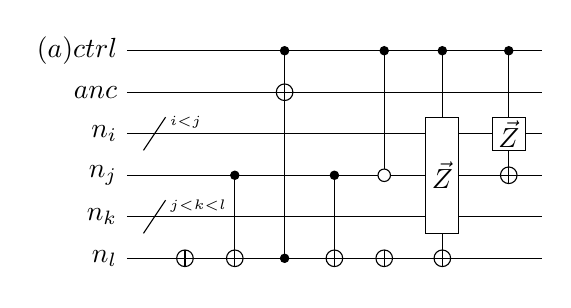
\begin{tikzpicture}[scale=1.000000,x=1pt,y=1pt]
\filldraw[color=white] (0.000000, -7.500000) rectangle (150.000000, 82.500000);
% Drawing wires
% Line 1: c W \text{(a) }ctrl
\draw[color=black] (0.000000,75.000000) -- (150.000000,75.000000);
\draw[color=black] (0.000000,75.000000) node[left] {$\text{(a) }ctrl$};
% Line 2: a W anc
\draw[color=black] (0.000000,60.000000) -- (150.000000,60.000000);
\draw[color=black] (0.000000,60.000000) node[left] {$anc$};
% Line 3: i W n_i
\draw[color=black] (0.000000,45.000000) -- (150.000000,45.000000);
\draw[color=black] (0.000000,45.000000) node[left] {$n_i$};
% Line 4: j W n_j
\draw[color=black] (0.000000,30.000000) -- (150.000000,30.000000);
\draw[color=black] (0.000000,30.000000) node[left] {$n_j$};
% Line 5: k W n_k
\draw[color=black] (0.000000,15.000000) -- (150.000000,15.000000);
\draw[color=black] (0.000000,15.000000) node[left] {$n_k$};
% Line 6: l W n_l
\draw[color=black] (0.000000,0.000000) -- (150.000000,0.000000);
\draw[color=black] (0.000000,0.000000) node[left] {$n_l$};
% Done with wires; drawing gates
% Line 8: i / ^{i<j}
\draw (6.000000, 39.000000) -- (14.000000, 51.000000);
\draw (12.000000, 48.000000) node[right] {$\scriptstyle{^{i<j}}$};
% Line 9: k / ^{j<k<l}
\draw (6.000000, 9.000000) -- (14.000000, 21.000000);
\draw (12.000000, 18.000000) node[right] {$\scriptstyle{^{j<k<l}}$};
% Line 10: c a i j k l LABEL width=-20
% Line 12: +l
\begin{scope}
\draw[fill=white] (21.000000, 0.000000) circle(3.000000pt);
\clip (21.000000, 0.000000) circle(3.000000pt);
\draw (18.000000, 0.000000) -- (24.000000, 0.000000);
\draw (21.000000, -3.000000) -- (21.000000, 3.000000);
\end{scope}
% Line 13: j +l
\draw (39.000000,30.000000) -- (39.000000,0.000000);
\filldraw (39.000000, 30.000000) circle(1.500000pt);
\begin{scope}
\draw[fill=white] (39.000000, 0.000000) circle(3.000000pt);
\clip (39.000000, 0.000000) circle(3.000000pt);
\draw (36.000000, 0.000000) -- (42.000000, 0.000000);
\draw (39.000000, -3.000000) -- (39.000000, 3.000000);
\end{scope}
% Line 14: c l +a
\draw (57.000000,75.000000) -- (57.000000,0.000000);
\filldraw (57.000000, 75.000000) circle(1.500000pt);
\filldraw (57.000000, 0.000000) circle(1.500000pt);
\begin{scope}
\draw[fill=white] (57.000000, 60.000000) circle(3.000000pt);
\clip (57.000000, 60.000000) circle(3.000000pt);
\draw (54.000000, 60.000000) -- (60.000000, 60.000000);
\draw (57.000000, 57.000000) -- (57.000000, 63.000000);
\end{scope}
% Line 15: j +l
\draw (75.000000,30.000000) -- (75.000000,0.000000);
\filldraw (75.000000, 30.000000) circle(1.500000pt);
\begin{scope}
\draw[fill=white] (75.000000, 0.000000) circle(3.000000pt);
\clip (75.000000, 0.000000) circle(3.000000pt);
\draw (72.000000, 0.000000) -- (78.000000, 0.000000);
\draw (75.000000, -3.000000) -- (75.000000, 3.000000);
\end{scope}
% Line 16: +l
\begin{scope}
\draw[fill=white] (93.000000, 0.000000) circle(3.000000pt);
\clip (93.000000, 0.000000) circle(3.000000pt);
\draw (90.000000, 0.000000) -- (96.000000, 0.000000);
\draw (93.000000, -3.000000) -- (93.000000, 3.000000);
\end{scope}
% Line 18: c -j
\draw (93.000000,75.000000) -- (93.000000,30.000000);
\filldraw (93.000000, 75.000000) circle(1.500000pt);
\draw[fill=white] (93.000000, 30.000000) circle(2.250000pt);
% Line 20: i j k G $\vec{Z}$ c +l
\draw (114.000000,75.000000) -- (114.000000,0.000000);
\begin{scope}
\draw[fill=white] (114.000000, 30.000000) +(-45.000000:8.485281pt and 29.698485pt) -- +(45.000000:8.485281pt and 29.698485pt) -- +(135.000000:8.485281pt and 29.698485pt) -- +(225.000000:8.485281pt and 29.698485pt) -- cycle;
\clip (114.000000, 30.000000) +(-45.000000:8.485281pt and 29.698485pt) -- +(45.000000:8.485281pt and 29.698485pt) -- +(135.000000:8.485281pt and 29.698485pt) -- +(225.000000:8.485281pt and 29.698485pt) -- cycle;
\draw (114.000000, 30.000000) node {$\vec{Z}$};
\end{scope}
\filldraw (114.000000, 75.000000) circle(1.500000pt);
\begin{scope}
\draw[fill=white] (114.000000, 0.000000) circle(3.000000pt);
\clip (114.000000, 0.000000) circle(3.000000pt);
\draw (111.000000, 0.000000) -- (117.000000, 0.000000);
\draw (114.000000, -3.000000) -- (114.000000, 3.000000);
\end{scope}
% Line 21: i G $\vec{Z}$ c +j
\draw (138.000000,75.000000) -- (138.000000,30.000000);
\begin{scope}
\draw[fill=white] (138.000000, 45.000000) +(-45.000000:8.485281pt and 8.485281pt) -- +(45.000000:8.485281pt and 8.485281pt) -- +(135.000000:8.485281pt and 8.485281pt) -- +(225.000000:8.485281pt and 8.485281pt) -- cycle;
\clip (138.000000, 45.000000) +(-45.000000:8.485281pt and 8.485281pt) -- +(45.000000:8.485281pt and 8.485281pt) -- +(135.000000:8.485281pt and 8.485281pt) -- +(225.000000:8.485281pt and 8.485281pt) -- cycle;
\draw (138.000000, 45.000000) node {$\vec{Z}$};
\end{scope}
\filldraw (138.000000, 75.000000) circle(1.500000pt);
\begin{scope}
\draw[fill=white] (138.000000, 30.000000) circle(3.000000pt);
\clip (138.000000, 30.000000) circle(3.000000pt);
\draw (135.000000, 30.000000) -- (141.000000, 30.000000);
\draw (138.000000, 27.000000) -- (138.000000, 33.000000);
\end{scope}
% Done with gates; drawing ending labels
% Done with ending labels; drawing cut lines and comments
% Done with comments
\end{tikzpicture}
